%!TEX root = ../dokumentation.tex

\chapter{Stand der Technik}
\section{Regelkreis Fahrzeug}
In einem Fahrzeug, das nicht autonom fährt, übernimmt der Fahrer die Aufgabe, die richtige Spur und Geschwindigkeit zu halten. Der Fahrer tritt somit als Regler auf. Zu den Aufgaben des Fahrers gehören neben der direkten Regelung die Planung der Fahrt. Dies beinhaltet die Wahl der geeigneten Strecke. Beispielsweise entscheidet der Fahrer, ob er sein Ziel besser über die Autobahn oder Landstraßen erreichen kann. Auf der Strecke muss der Fahrer in der Lage sein, dynamisch auf Hindernisse wie beispielsweise Baustellen, Straßensperren und Kreuzungen reagieren \cite{MIT15}.

Die menschliche Informationsverarbeitung bietet sich offensichtlich für den Entwurf eines autonom fahrenden Systems an. Rasmussen unterteilt in \cite{RAS83} das Verhalten eines Menschen in drei verschiedene Ebenen. Dies ist in Abbildung \ref{RAS:INF} veranschaulicht. Unter Fertigkeiten ordnet Rasmussen stark automatisiertes Verhalten ein. Der Mensch muss hierbei nicht besonders aufmerksam sein. Aktionen die auf dieser Verhaltensebene durchgeführt werden als regelbasiertes Verhalten beschrieben. In Situationen die unbekannt sind, wird, nach Rasmussen, auf wissensbasierte Verhaltensweisen zurückgegriffen. Dieses Modell dient als Grundlage für viele weitere Theorien und kann für den Entwurf von Agenten für das autonome Fahren verwendet werden.
\FloatBarrier
\begin{figure}[h]
  \centering
  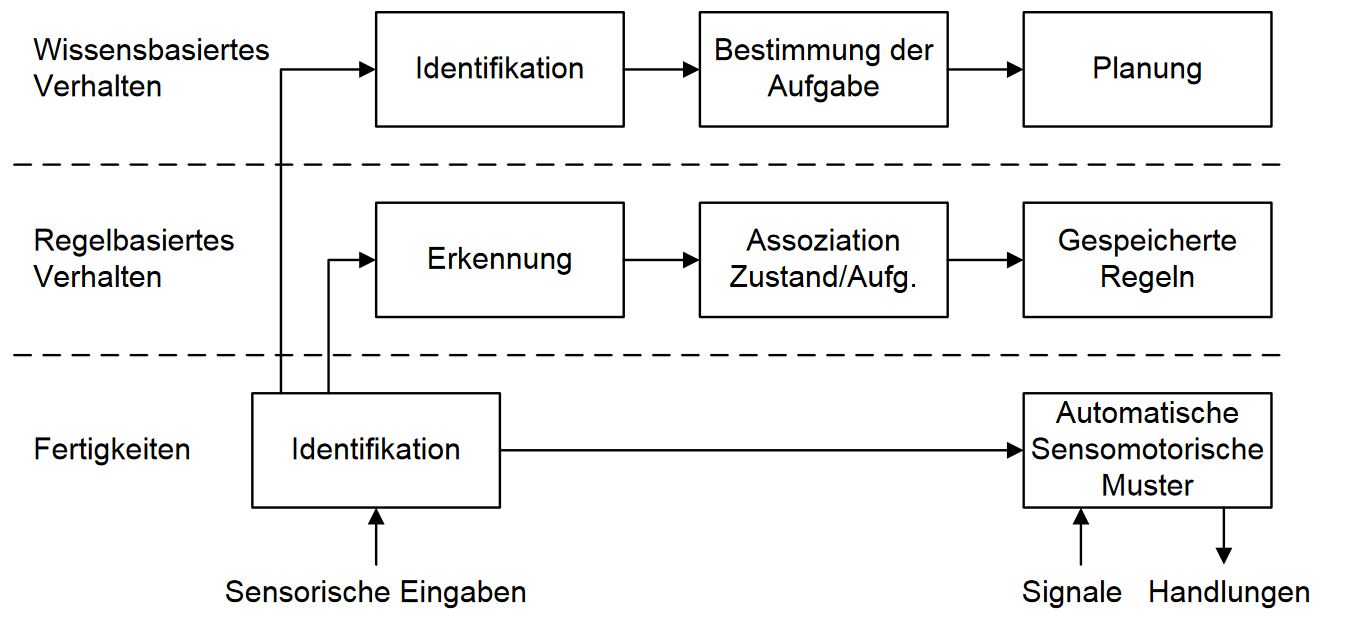
\includegraphics[width=0.9\textwidth]{images/stand_der_technik/Rasmussen.JPG}
  \caption[Informationsverarbeitung nach Rasmussen]{Informationsverarbeitung nach Rasmussen \cite{RAS83}}
  \label{RAS:INF}
\end{figure}
\FloatBarrier

\section{Das autonome Fahrzeug als kognitives System}
Nach \cite{TAS16} kann ein autonomes Fahrzeug genauso wie ein Mensch als kognitives System betrachtet werden. Dieses System lässt sich in drei Komponenten gliedern. Diese sind in Abbildung \ref{kog:sys} gezeigt. Das Perzeptions-Modul verarbeitet die Daten der Sensoren. Dazu gehören unter anderem die Lokalisierung des Fahrzeugs und die Erkennung von relevanten Objekten. Diese Informationen werden an das kognitive Entscheidungs System weitergeleitet. Dieses entscheidet und plant, welche Aktionen durchgeführt werden sollen. Die Durchführung der ausgewählten Aktion wird von der Komponente Aktion übernommen. Dieses regelt beziehungsweise steuert die Aktoren des Autonomen Fahrzeugs. Das gesamte Fahrzeug steht damit in einem Regelkreis mit der Umgebung.
\FloatBarrier
\begin{figure}[h]
  \centering
  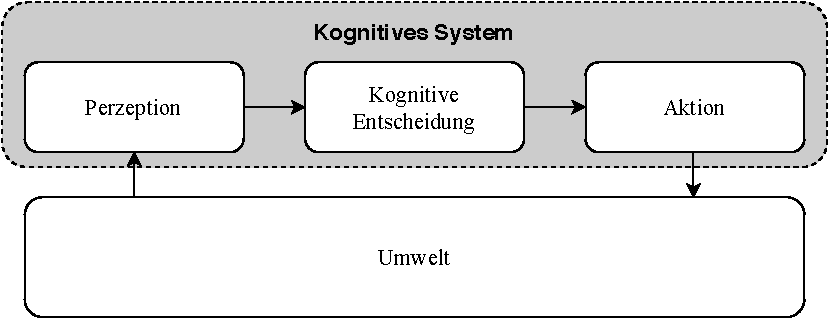
\includegraphics[width=0.8\textwidth]{images/stand_der_technik/kognitivesSystem.pdf}
  \caption[Aufbau eines kognitiven Systems]{Aufbau eines kognitiven Systems}
  \label{kog:sys}
\end{figure}
\FloatBarrier

\section{Bestehende Ansätze zur Strukturierung der Software für autonome Fahrzeuge}
Es bestehen unterschiedliche Ansätze, ein Software-System für autonome Fahrzeuge zu gestalten. Nach \cite{JUN14} unterscheiden sich grundsätzlich zwei verschiedene Ansätze. Zum einen die hierarchische Struktur und zum anderen die parallele Struktur. Zudem wird eine manöverbasierte Struktur vorgestellt.

\subsection{Hierarchische Struktur}
Hierarchische Strukturen bestehen aus Modulen die in verschiedenen Ebenen angeordnet sind. Auf jeder Ebene wird die Eingabe, die Mission, der nächsthöheren Ebene in Submissionen aufgeteilt und an die unterliegende Schicht weitergegeben.

Abbildung \ref{abb:hir} zeigt die Umsetzung einer solchen Struktur. Das Perzeptionssystem analysiert in Echtzeit die Eingaben von Lidar, Kamera und anderen Sensoren. Das Mission planning System generiert dabei einen Weg mit Zwischenzielen. Dabei wird die Ankunftszeit, benötigte  Manöver und die Distanz berücksichtigt. Das Behavior executive System fällt Entscheidungen über taktische Fahrmanöver wie Überholmanöver, Spurwechsel oder Interaktionen mit anderen Fahrzeugen. Im Motion planning Modul wird dann die endgültige Trajektorie errechnet. Dabei werden insbesondere der gewünschte  Lenkwinkel und die gewünschte Gaspedalstellung festgelegt.

Nach \cite{JUN14} ist ein Nachteil dieser Architektur, dass hierarchisch hoch oben angesiedelte Module nicht genügend Informationen haben und weiter unten angesiedelte Module nicht die Autorität die bereits getroffenen Entscheidungen zu redigieren.
\FloatBarrier
\begin{figure}[h]
  \centering
  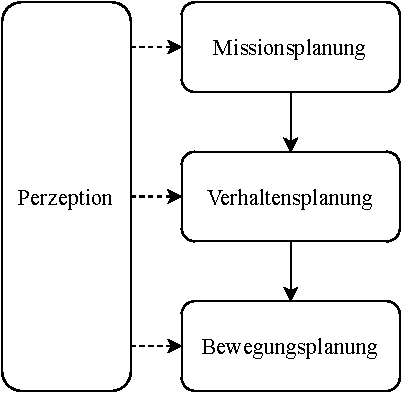
\includegraphics[width=0.5\textwidth]{images/stand_der_technik/hierarchische_struktur.pdf}
  \caption[Hierarchische Softwarestrukur f\"ur autonome Fahrzeuge]{Hierarchische Softwarestrukur f\"ur autonome Fahrzeuge nach \cite{JUN14}}
  \label{abb:hir}
\end{figure}
\FloatBarrier
\subsection{Parallele Struktur}
Die parallele Struktur verfolgt den Ansatz, verschiedene Module gleichzeitig auszuführen. In Abbildung \ref{par:str} ist dies gezeigt. Die Regler Module arbeiten unabhängig voneinander und verwenden zur Berechnung die Daten des Perzeptions Moduls. Oftmals sind dabei eigene Sensoren für jeden Regler vorgesehen. Der Vorteil ist hierbei, dass die Regler unabhängig voneinander ausgelegt und ausgetauscht werden können. Problematisch sind hierbei jedoch die Ausführung von sehr komplexen Fahrmanövern, da die Regler nicht aufeinander abgestimmt sind \cite{JUN14}. Zudem ist es oftmals nur schwer möglich, diese System zu erweitern, da dafür meist jedes Modul angepasst werden muss.
\FloatBarrier
\begin{figure}[t]
  \centering
  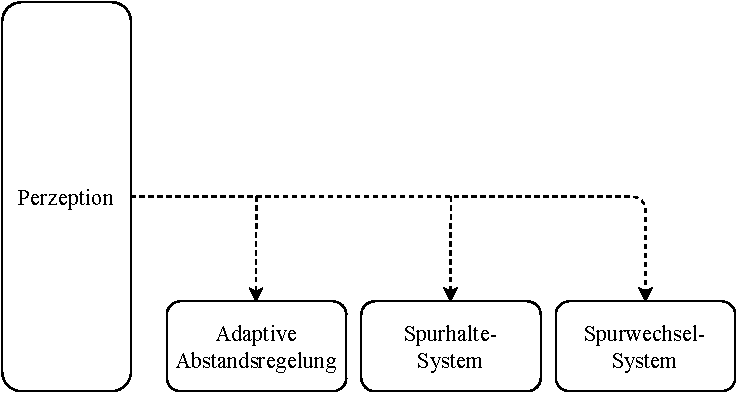
\includegraphics[width=\textwidth]{images/stand_der_technik/parallele_struktur.pdf}
  \caption[Parallele Softwarestruktur für autonome Fahrzeuge]{Parallele Softwarestruktur für autonome Fahrzeuge nach \cite{JUN14}}
  \label{par:str}
\end{figure}
\FloatBarrier

\subsection{Manöverbasierte Struktur}
In \cite{DUA20} wird eine manöverbasierte Softwarestruktur für eine autonomes Fahrzeug vorgestellt. Diese Softwarestruktur basiert auf neuronalen Netzwerken, die in Modulen ausgeführt werden. Jedes Modul ist für die Ausführung eines Manövers zuständig. Ein Manöver kann beispielsweise ein Spurwechsel, ein Einparkvorgang oder das Halten an einer Kreuzung sein. Diese Manöver werden jeweils vom zugehörigen Modul durchgeführt. Ein weiteres Modul entscheidet, welches Manöver im Moment durchgeführt werden soll. Das Fahrzeug führt zu jedem Zeitpunkt ein Manöver aus. Es handelt sich somit bei dieser Software-Struktur auch um eine hierarchische Struktur nach \cite{JUN14}.

In \cite{DUA20} wird beschrieben, dass beim Übergang zwischen Manövern Sprünge auf den Ausgangssignalen für die Aktoren im Fahrzeug entstehen können. Dies äußert sich als ruckartige Bewegung im Fahrzeug und kann besonders während dem Fahren gefährlich werden. Der Vorteil dieser Struktur ist insbesondere, dass die Module unabhängig voneinander entwickelt werden können. Zudem können die Module sehr leicht ausgetauscht werden. Darüber hinaus kann das Verhalten an komplexere Umgebungen angepasst werden, indem weitere Module für bestimmte Manöver hinzugefügt werden.

\FloatBarrier
\begin{figure}[h]
  \centering
  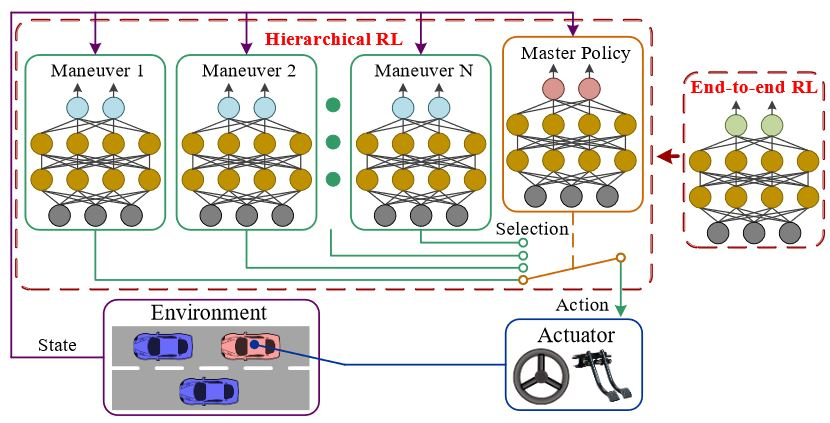
\includegraphics[width=\textwidth]{images/stand_der_technik/NN_SW_Structure.JPG}
  \caption[Manöverbasierte Softwarestruktur für autonome Robotor]{Manöverbasierte Struktur für autonome Robotor nach \cite{DUA20}}
  \label{NN:SW}
\end{figure}
\FloatBarrier

\section{Modellierung von Verhaltensweisen}
Die Informatik bietet verschiedene Möglichkeiten Verhaltensweisen zu modellieren. Diese sind im Bereich des autonomen Fahrens relevant, um die Verhaltenssteuerung der Fahrzeuge zu realisieren.

\subsection{Finite deterministische Zustandsautomaten}
Zustandsautomaten (kurz FSM) werden in der Informatik verwendet um Protokolle oder Verhaltensweisen zu beschreiben. Ein Zustandsautomat wird durch ein 5-Tupel $\mathcal{A} = (Q, \Sigma, \delta, q_0, F)$ definiert. Diese Bestandteile sind wie folgt definiert:
\begin{itemize}
 \item $Q$ einer Menge von Zuständen $q_i$
 \item $\Sigma$ einem Eingabealphabet
 \item $\delta(q, a)=q': Q \times \Sigma \rightarrow Q$ eine Transitions- oder Übergangsfunktion, die einen Zustand in einen anderen überführt
 \item $q_0 \in Q$ dem Startzustand
 \item $F \subset Q$ der Endzustandsmenge
\end{itemize}

Die Wartung von Zustandsautomaten ist aufwändig, wenn Zustände oft hinzugefügt oder entfernt werden sollen. Es wird dann notwendig eine große Anzahl von Übergängen zwischen Zuständen einzufügen oder zu löschen. Dabei besteht die Möglichkeit, dass Fehler passieren die übersehen werden. Besonders große Zustandsautomaten sind oftmals schlecht zu überblicken. 

\subsection{Hierarchische Zustandsautomaten}
Das Modell der Hierarchischen Zustandsautomaten (engl. Hierarchical State Machines, kurz HFSM) ist ein erweitertes Model der FSM. HFSM erlauben die Schachtelung von Zuständen und somit Subautomaten und Subzustände zu bilden.  

In einem HFSM existiert immer ein Top-Zustand. Dieser ist der oberste Zustand im Modell. Anderen Zustände können Subzustände dieses Top-Zustands sein. Zustände können beliebig tief verschachteltet werden. Wenn ein Subzustand aktiv ist bedeutet dies, dass alle Top-Zustände auch aktiv sind. Der Zustand, der direkt über dem relevanten Subzustand liegt, wird Super-Zustand genannt. 
HFSM eignen sich besonders für die Modellierung komplexer Verhaltensweisen. Ein einfacher HFSM ist in Abbildung \ref{HFS:PLC} gezeigt. Dieser HFSM besteht aus zwei Super-Zuständen mit jeweils zwei Sub-Zuständen.
\FloatBarrier
\begin{figure}[h]
  \centering
  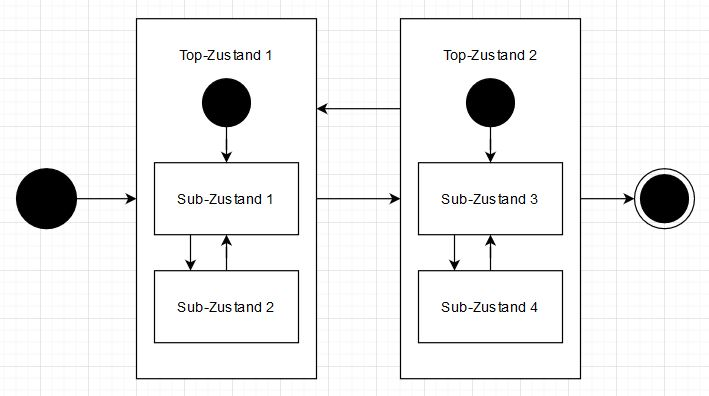
\includegraphics[width=0.7\textwidth]{images/stand_der_technik/HFSM_Plazebo.JPG}
  \caption[Finiter endlicher Zustandsautomat]{Finiter endlicher Zustandsautomat}
  \label{HFS:PLC}
\end{figure}
\FloatBarrier

\subsection{Verhaltensbäume}
Verhaltensbäume werden insbesondere in der Computerspiele-Industrie verwendet, um das Verhalten von Agenten zu beschreiben. Das Grundkonzept beruht darauf, dass elementare Aktionen auf denen die Verhaltensweise basiert, baumartig strukturiert sind.

Die Ausführung eines Verhaltensbaums erlaubt keine Speicherung von Zuständen. Dies gestaltet die Ausführung von Sequenzen sehr schwierig die länger als die Zwischenzeit zwischen den einzelnen "Ticks" dauert. Daraus  resultiert insbesondere ein Problem wenn eine bestimmte Sequenz über mehrere \"Ticks\" ausgeführt werden soll. Es kann somit passieren, dass die Ausführung einer Sequenz unterbrochen wird, obwohl eine andere Aktion im Moment ausgeführt werden soll. In \cite{KLC15} wird ein Ansatz, vorgestellt einen Verhaltensbaum mit einem Speicher für Zustände zu realisieren vorgestellt. Dabei geht jedoch auch ein Teil die Übersichtlichkeit des Baums verloren. Bei sehr großen Verhaltensbäumen können Laufzeitprobleme auftreten, da der Baum immer von der Wurzel durchlaufen wird. 

\subsection{Neuronale Netze}
Das Konzept von künstlicher Intelligenz mit neuronalen Netzen ist am menschlichen Gehirn orientiert. Besonders in den letzten Jahren konnten mithilfe von neuronalen Netze Durchbrüche in der Bilderkennung [XYZ] und der Robotik [XYZ] erreicht worden. Grigorescu et. al. beschreiben in \cite{GRI19}, dass künstliche Intelligenz durch neuronale Netze zur Verhaltenssteuerung in autonomen Fahrzeugen bereits in Projekten wie beispielsweise der DARPA challenge 2017 erfolgreich eingesetzt wurden. In \cite{MIR18} wird beispielsweise ein Verfahren vorgestellt, das es erlaubt mithilfe eines neuronalen Netzes zu entscheiden, ob ein Überholvorgang eingeleitet werden kann. Hier wird gezeigt, dass es möglich ist, mit diesem Ansatz in Fahrzeugen Entscheidungen autonom zu treffen. 

Ein neuronales Netz wird analog zu einem Graphen über eine Menge an Kanten und Knoten also Neuronen und Verbindungen definiert. Jede Verbindung hat ein Gewicht und jedes Neuron einen Bias. Zusätzlich wird eine Aktivierungsfunktion für jedes Neuron definiert \cite{CIT11}.

Die Netzwerke müssen vor dem Einsatz angelernt werden. Dazu ist die Verwendung einer Simulationsumgebung notwendig, da so Testfahrten sicher durchgeführt werden können. Zusätzlich können Tests so automatisiert durchgeführt werden. Dies erlaubt es das Netzwerk schnell anzupassen, da die meisten Simulationen die Realität nicht genügend genau abbilden. Daher kann es passieren, dass die in der Simulation erprobten neuronalen Netze nicht direkt auf eine reale Umgebung anwendbar sind \cite{GRI19}. Zusätzlich stellt die Realisierung einer detailgetreuen Simulationsumgebung meist einen sehr hohen Arbeitsaufwand dar. Aufgrund der hohen Komplexität größerer neuronaler Netze ist die Verhaltensweise oftmals nur schwer nachvollziehbar. Besonders das zuvor beschriebene eigenständige Erlernen bestimmter typischer Verhaltensweisen kann zu Problemen führen. Um die Sicherheit zu gewährleisten, sollten nach \cite{GRI19} zusätzliche Sicherheitsmaßnahmen wie beispielsweise Watchdogs etc. erwogen werden. Damit soll das Fahrzeug im Zweifel in einen sicheren Zustand überführt werden. Ein Nachweis über die funktionale Sicherheit des Systems müsste daher durch Statistiken, die über viele Fahrstunden erstellt werden. 

\section{Betriebssysteme}
Autonom fahrende Fahrzeuge verfügen oftmals über ein Zentralsteuergerät zur Ausführung komplexer Aufgaben. Dieses Zentralsteuergerät verfügt zumeist über ein Betriebssystem. Zu den Aufgaben des Betriebssystems gehört die Verteilung der Rechenzeit unter den einzelnen Prozessen, die Anbindung von Peripheriegeräten und die Bereitstellung von grundlegenden Diensten. Die Alternative zur Verwendung eine Betriebssystems ist der Aufbau eines monolithischen Softwaresystems. Je nachdem wie komplex und groß das Softwaresystem wird, kann dies sehr kompliziert zu warten und zu erweitern werden.

\subsection{Robot Operating System}
Das Robot Operating System (kurz ROS) ist ein open-source Software-Framework, das die Entwicklung komplexer modularer Softwaresysteme für Roboter unterstützt. ROS benötigt zur Ausführung zusätzlich ein zugrundeliegendes Linux Betriebssystem. Applikationen, die auf ROS aufsetzen, können in C++ oder Python geschrieben werden. ROS übernimmt die Kommunikation zwischen einzelnen Softwaremodulen und bietet eine Vielzahl an bestehenden Erweiterungen an. Anwendungen können mithilfe von ROS auf verschiedene Rechner aufgeteilt werden \cite{AND16}.

Systeme, die auf dem Robot Operating Systems basieren, bestehen meist aus mehreren einzelnen Modulen, sogenannte \textit{Nodes} oder \textit{Nodelets}. Diese Module können auf verschiedenen Wegen miteinander kommunizieren. Die Kommunikation wird von einem Master Server verwaltet.  
In Abbildung \ref{ros:str} ist zu sehen, dass dieser Server auch \textit{Nodes} ausführen kann. Weitere Slave Server können ihre \textit{Nodes} beim Master registrieren und werden somit serverübergreifend erreichbar. Zur Kommunikation zwischen den Servern wird das TCP oder UDP Protokoll verwendet.
\FloatBarrier
\begin{figure}[h]
  \centering
  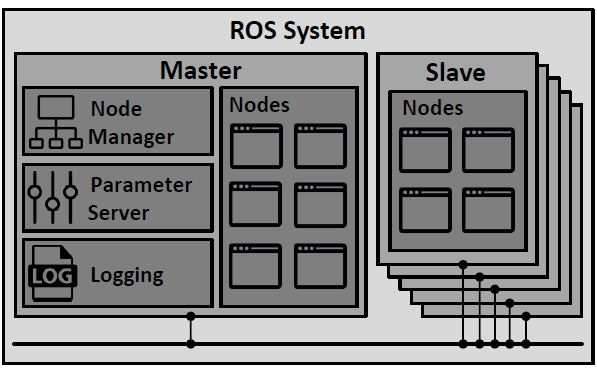
\includegraphics[width=\textwidth]{images/stand_der_technik/ROS_AS.JPG}
  \caption[Struktur des Robot Operating System]{Struktur des Robot Operating System}
  \label{ros:str}
\end{figure}
\FloatBarrier
Nachrichtentypen können ähnlich wie Objekte in C++ in ROS beschrieben werden. Darüber hinaus stehen dem Anwender einige Grundtypen zur Verfügung. Diese Grundtypen decken sich mit weitestgehend den Datentypen in C++ \cite{AND16}.

Die Kommunikation zwischen den \textit{Nodes} erfolgt über das Publish/Subscribe-Prinzip. Dies bedeutet, dass Nodes sogenannte Topics mit einem bestimmten Nachrichtentyp beim Master registrieren können. Alle angebundenen Nodes können daraufhin diesem Topic subscriben und erhalten dann immer die zuletzt gesendete Nachricht auf diesem bestimmten Topic. Es können auch mehr als ein Node auf einem bestimmten Topic publischen.

\subsection{Automotive Data and Time-Triggered Framework}
Das Automotive Data and Time-Triggered Framework (ADTF) ist eine propietäre Software die von der Firma Elektrobit vermarktet wird. Es ist ein Echtzeitsystem und wird zur Entwicklung von sogenannten Advanced Driver Assistance Systemen (ADAS) verwendet. Die Software unterstützt das synchrone und asynchrone Verarbeiten von Daten. Es ermöglicht die Erprobung der Software in Simulationsumgebung und die Programmierung von Softwarebestandteilen in C und C++. Darüber hinaus können über Toolboxen Programmierumgebungen wie Matlab/Simulink angebunden werden. Da ADTF ein professionell lizenziertes Produkt ist wird es hauptsächlich von Unternehmen verwendet. Die Community des ADTF ist daher nur sehr klein \cite{AND16}.

\section{Aufbau des Fahrzeugs der DHBW Smart Rollerz}
Das Fahrzeug verfügt über einen Elektromotor, der über ein Getriebe mit allen Rädern verbunden ist. Darüber hinaus wird ein Servomotor verwendet, um die Vorderräder zu lenken. Zusätzlich sind Lichter am Fahrzeug angebracht. Diese dienen dazu, Manöver korrekt anzuzeigen und die Verwendung der Fernbedienung durch eine leuchtende blaue LED zu signalisieren. In Abbildung \ref{sen:zeg} ist das aufgebaute autonom fahrende Fahrzeug zu sehen.

\FloatBarrier
\begin{figure}[h]
  \centering
  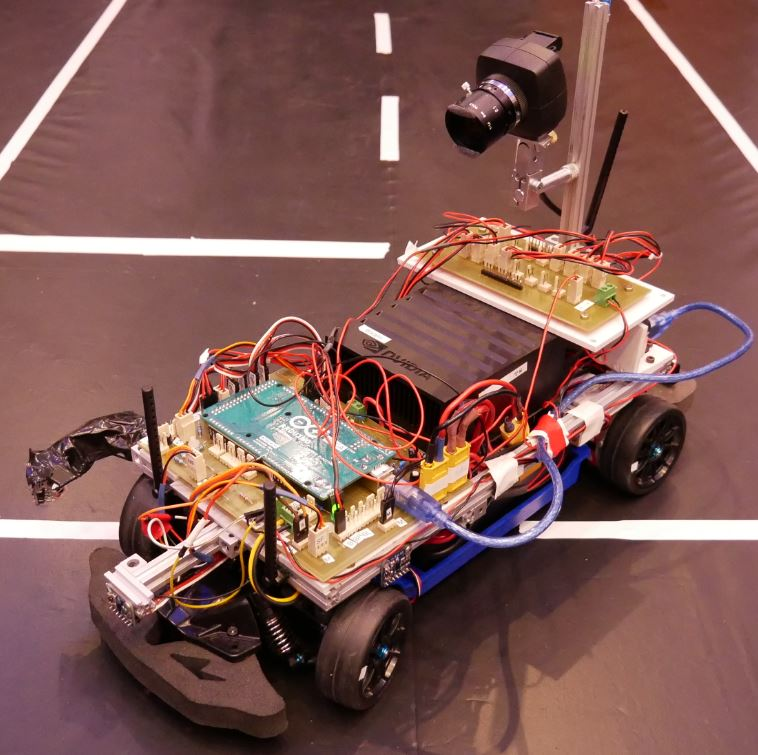
\includegraphics[width=0.5\textwidth]{images/stand_der_technik/SR_Fahrzeug.JPG}
  \caption[Fahrzeug der DHBW Smart Rollerz]{Fahrzeug der DHBW Smart Rollerz}
  \label{sen:zeg}
\end{figure}
\FloatBarrier

Das Fahrzeug verfügt über verschiedene Sensoren, um die Umgebung des Fahrzeugs zu erkennen. Ein Überblick über die angebrachten Sensoren gibt Abbildung \ref{sen:auf}. Die Kamera wird 30 Zentimeter über dem Fahrzeug montiert und ist nach vorne gerichtet. Dies soll es ermöglichen, die Spuren der Fahrbahn, Kreuzungen, Parkplätze und die Startlinie zu erkennen. Zusätzlich sind drei Distanzsensoren am Fahrzeug angebracht. Sie haben einen Messbereich von etwa 3 Zentimetern zu einem Meter. Der nach vorne gerichtete Distanzsensor soll vorrausfahrende Fahrzeuge erkennen. Um Vorfahrtssituationen zu erkennen wird ein schräg nach vorne gerichteter Sensor verwendet. Der seitlich angebrachte Distanzsensor kommt beim Erkennen und Vermessen von Parklücken als auch bei Überholvorgängen zum Einsatz. Zur Bestimmung der Geschwindigkeit verfügt das Fahrzeug zudem über einen Drehzahlsensor und einen Beschleunigungsmesser. Der Beschleunigungsmesser soll es ermöglichen, die Geschwindigkeit genauer zu ermitteln und die Kurvenbeschleunigung für die Regelung zu messen.

\FloatBarrier
\begin{figure}[h]
  \centering
  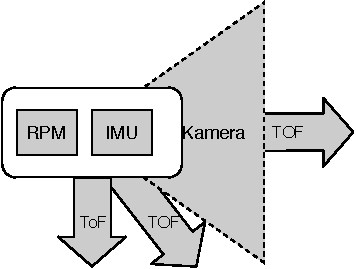
\includegraphics[width=0.3\textwidth]{images/stand_der_technik/Sensoren.pdf}
  \caption[Sensorik des aufgebauten Fahrzeugs]{Sensorik des aufgebauten Fahrzeugs}
  \label{sen:auf}
\end{figure}
\FloatBarrier